\documentclass[11pt,a4paper]{report}
\usepackage[top=1in, bottom=1.5in, left=1in, right=1in]{geometry}
\usepackage[utf8]{inputenc}
\usepackage{amsmath}
\usepackage{amsfonts}
\usepackage{amssymb}
\usepackage[spanish,activeacute]{babel}
\usepackage{multirow}
\usepackage{graphicx}
\usepackage{setspace}
\usepackage{color}
\definecolor{red}{rgb}{1,0,0}
\newcommand\red[1]{\textcolor{red}{#1}}
\newcommand{\dsum}{\displaystyle\sum}

\begin{document}

\setlength{\unitlength}{1 cm} %Especificar unidad de trabajo
\thispagestyle{empty}
\begin{picture}(18,4)
\put(0,0){
\includegraphics[width=2.3cm,height=3cm]{LOGO.jpg}}
%\put(11.5,0){\includegraphics[width=4cm,height=4cm]{eupinf.jpg}}
\end{picture}
\begin{center}
\textbf{{\LARGE Universidad de Concepci\'on}}\\[0.5cm]
{\Large Facultad de Ciencias F\'isicas y Matem\'aticas}\\[0.5cm]
{\Large Departamento de Estad\'istica}\\[3.5cm]
{\LARGE \textbf{LABORATORIO III}}\\[1cm]
{\LARGE \textbf{DATA MINING}}\\ [4cm]
{\large Nombres: Katerin De la hoz Luna}\\
\hspace{2.2cm}{\large Fernando Pe\~na Villalobos}\\
\hspace{1.7cm}{\large Ariel P\'erez Almonacid}\\[2cm]

{\large Concepci\'on \\
\today}
\end{center}

\newpage

\begin{center}
{\large TRABAJO}
\end{center}

\begin{itemize}
\item[1.]
Consideremos los siguientes 4 individuos  $A_{1}$, $A_{2}$, $A_{3}$ y $A_{4}$ y su matriz de distancias

$$\begin{tabular}{| c | l c r r |}
\hline
 &  $A_{1}$ & $A_{2}$ & $A_{3}$ & $A_{4}$  \\
 \hline  
 $A_{1}$ & 0 & 5 & 2 & 3 \\
 $A_{2}$&  & 0 & 1 & 7\\
 $A_{3}$&  &  &  0& 6\\
 $A_{4}$&  &  &  &0\\
   \hline
 \end{tabular} $$
\begin{enumerate}
\item[i)] Agregación de salto máximo:

$$\delta_{\max}(x,y)=\max\{  d(x,k): \ \ h\in x, \ k\in y\}$$
Donde $d$ es la distancia euclideana.\\
Primero notamos que los que están más cerca son $A_{2}$  y $A_{3}$. Luego, utilizando salto máximo:

$$\begin{tabular}{| c | l  r r |}
\hline
 &  $A_{1}$ & $\{A_{2},A_{3}\}$ & $A_{4}$  \\
 \hline  
 $A_{1}$ & 0 & 5  &  3 \\
 $\{A_{2},A_{3}\}$&  & 0 &  7\\
 $A_{4}$  &  &    &0\\
   \hline
 \end{tabular} $$
Notamos que $A_{1}$ y $A_{4}$ son los más cercanos, así que los juntaremos en un clúster y $ \delta_{\max}(\{A_{2},A_{3}\},\{A_{1},A_{4}\})=7$
$\Longrightarrow$ La matriz de clasificación binaria resulta ser:

$$\begin{tabular}{| c |   r r |}
\hline
   &    $\{A_{1},A_{4}\}$ & $\{A_{2},A_{3}\}$   \\
   \hline
 $\{A_{1},A_{4}\}$ & 0  &  7 \\
 $\{A_{2},A_{3}\}$ & & 0\\
   \hline
 \end{tabular} $$


\item[ii)] Agregación Promedio:

$$\delta_{\text{promedio}}(x,y)=\frac{1}{|x||y|}\dsum\{  d(x,k): \ \ h\in x, \ k\in y\}$$
Como es la misma tabla, los que están más cerca son $A_{2}$  y $A_{3}$. Así, utilizando agregación promedio:
$$\begin{tabular}{| c | l  r r |}
\hline
 &  $A_{1}$ & $\{A_{2},A_{3}\}$ & $A_{4}$  \\
 \hline  
 $A_{1}$ & 0 & 3,5  &  3 \\
 $\{A_{2},A_{3}\}$&  & 0 & 6,5  \\
 $A_{4}$  &  &    &0\\
   \hline
 \end{tabular} $$
Nuevamente, $A_{1} \text{ y }A_{4}$ son los más cercanos en distancia. Además,
$$\delta_{\text{promedio}}(\{A_{1},A_{4}\},\{A_{2},A_{3}\})=\frac{1}{2\cdot 2}(5+2+7+6)=20/4=5$$
$\Longrightarrow$ La matriz de clasificación binaria es de la forma:

$$\begin{tabular}{| c |   r r |}
\hline
   &    $\{A_{1},A_{4}\}$ & $\{A_{2},A_{3}\}$   \\
   \hline
 $\{A_{1},A_{4}\}$ & 0  &  5 \\
 $\{A_{2},A_{3}\}$ & & 0\\
   \hline
 \end{tabular} $$
 \end{enumerate}
\item[2.]
\begin{verbatim}
wss <- function(d) {
  sum(scale(d, scale = FALSE)^2) 
} 
#Hace la suma del cuadrado de las diferencias de cada dato 
#con el promedios
#esta formula hace alusión a la inercia intra-clases

wrap <- function(i, hc, x) {
  cl <- cutree(hc, i) 
  #Dado un árbol hc resultante de hclust, cutree corta el árbol 
  #en la cantidad de grupos deseados dados por i.
  #si i es escalar, entonces cutree entrega un vector con asignación de 
  #cada individuo a un grupo
  #si i es un vector, entonces cutree entrega una matriz donde cada 
  #columna j corresponde al elemento j de i, y la correspondiente 
  #asignación de cada individuo a un grupo.
  spl <- split(x, cl)
  #Divide el arreglo x en grupos definidos por cl
  #split entrega las listas que contienen los valores 
  #asociados para cada grupo.
  wss <- sum(sapply(spl, wss))
  #Aplica wss a spl, con lo cual se obtiene un vector con los valores 
  #de wss a cada lista de spl. Luego suma éstos.
  #Esta corresponde exactamente a la inercia intra-clases.
  wss
}
iris2 <- iris[, 1:4] 
#Extrae desde la primera hasta la cuarta columna
#del conjunto de datos iris que trae incorporado R.
cl <- hclust(dist(iris2), method = "ward.D")
#dist(iris2): matriz de distancias
#hace hclust con el método ward
res <- sapply(seq.int(1, nrow(iris2)), wrap, hc = cl, x = iris2)
#Aplica la función wrap a los siguientes parámetros
#i=seq.int(1, nrow(iris2)), hc=cl, x=iris .
#Primero corta al árbol en 1 a 150 grupos y lo guarda en cl
#que es una matriz de 150 por i, donde cada componente de ella
#tiene como valor el grupo al cual pertenece el individuo.
#Luego separa los datos de la tabla iris2 con respecto a cada grupo
#y los guarda como lista en spl (una lista por cada grupo).
#Por último calcula la inercia intra-clases (wss) para cada valor 
#de grupos a considerar (de 1 a 150).
#La variable res es un vector de largo 150 contiene los valores de las 
#inercias intra-clases para cada caso.
plot(seq_along(res), res, type = "b", pch = 19)
#Grafica la cantidad de grupos (1 a 150) versus la 
#inercia intra-clases
plot(seq_along(res[1:50]), res[1:50], type = "o", pch = 19)
#Grafica la cantidad de grupos (1 a 50) versus la
#inercia intra-clases
\end{verbatim}
\item[3.]

\begin{itemize}
\item[3.2)] Se utiliza análisis de componentes principales y se observa que con las primeras dos componentes se representa cerca de un $70\%$ de la información, por lo que es suficiente con usar sólo esas dos primeras.
\begin{center}
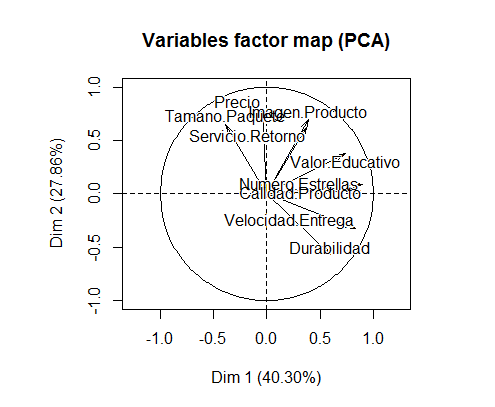
\includegraphics[scale=0.7]{Circulo.png}
\end{center}
Luego se procede a clusterizar en 2 y 3 grupos.
\begin{center}
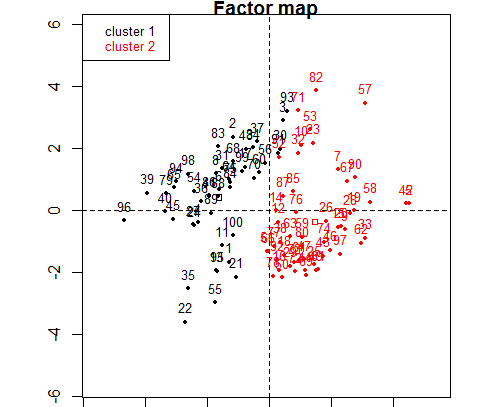
\includegraphics[scale=0.5]{hc2.png}
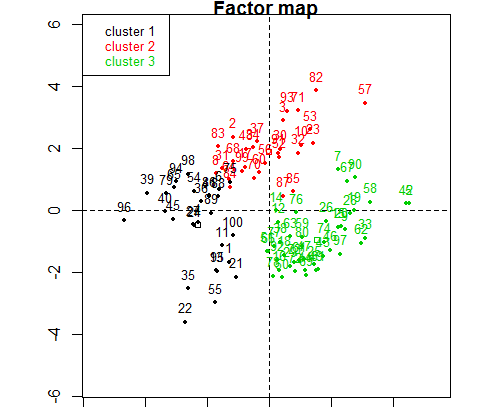
\includegraphics[scale=0.5]{hc3.png}
\end{center}
Utilizando el círculo de correlación, se observa que en la separación en dos grupos se agrupó en un clúster a aquellos que evalúan bien la velocidad de entrega, durabilidad, calidad de producto, número de estrellas, valor educativo, imagen de producto o servicio de retorno, junto con aquellos que evalúan mal el precio o el tamaño de paquete. Mientras que en el otro se agruparon a aquellos que evalúan bien precio y tamaño de paquete o que evaluaron mal alguna de las otras. Si bien se puede decir que los que evalúan bien durabilidad suelen coincidir con los que evalúan velocidad de entrega, los de número de estrellas con los de calidad de producto y valor educativo, los de imagen producto con los de servicio de retorno y los de precio con los tamaño de paquete; no se puede afirmar una relación, por ejemplo, entre valor educativo y durabilidad (lo mismo con todos aquellos cuyas flechas formen ángulos entre 50 y 130 grados). \\
\\
Por otro lado, se puede afirmar que aquellos que evalúan bien precio y tamaño de paquete suelen evaluar mal velocidad de entrega y durabilidad.\\
\\
Volviendo a los clústers, en la separación en tres grupos se dejó en uno a aquellos que evalúan bien durabilidad, velocidad de entrega, número de estrellas, calidad de producto y valor educativo con los que evalúan mal precio y tamaño de paquete. En otro se dejó a aquellos que evalúan bien imagen de producto, precio, servicio de retorno y tamaño de paquete. Y en el tercero a quienes evalúan mal imagen de producto, servicio de entrega, valor educativo, número de estrellas o calidad de producto.\\
\\
Además, en el siguiente gráfico se pueden observar los centros de gravedad de cada clúster, representado por un cuadrado.
\begin{center}
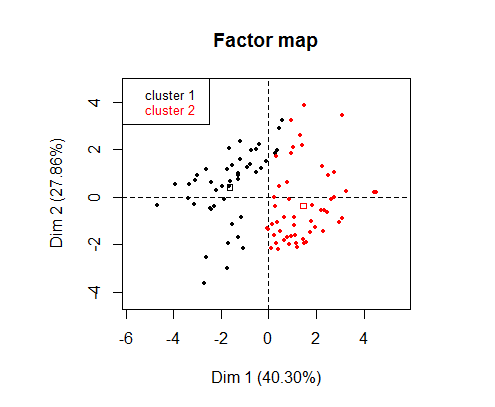
\includegraphics[scale=0.8]{centro2.png}
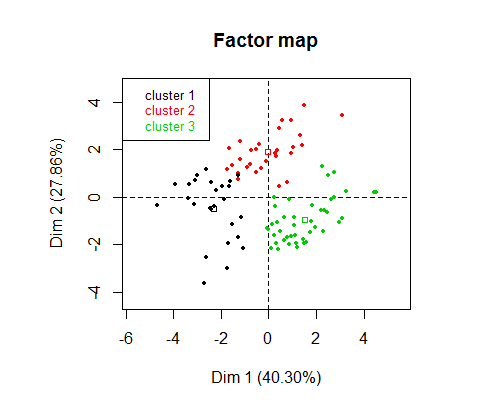
\includegraphics[scale=0.8]{centro3.png}
\end{center}

\item[3.3)] Utilizando hclust con el método de Ward, se obtiene el siguiente árbol:
\begin{center}
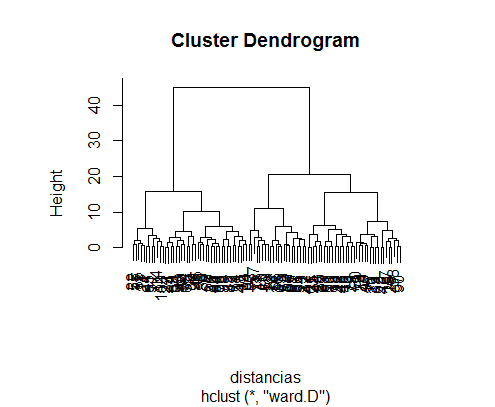
\includegraphics[scale=0.8]{hclust.png}
\end{center}
\item[3.4)-3.5)] Como en el gráfico anterior no se ve bien la división, se podará el árbol con la función cutree. Para lo cual, primero veremos cuál será el número más conveniente de grupos a considerar, graficando la inercia intra-clases versus el número de clases.
\begin{center}
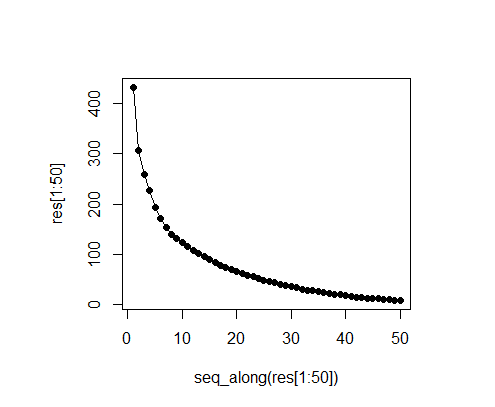
\includegraphics[scale=0.8]{codo.png}
\end{center}
Gracias al codo, se puede decir que el número ideal es siete. Sin embargo, tampoco se puede decir que estos grupos estarán muy bien definidos, pero ir separando en más clústers tampoco ayudaría de mucho, a menos que sean demasiados, con lo que se terminaría sobreajustando la clusterización a nuestros datos.\\
\begin{center}
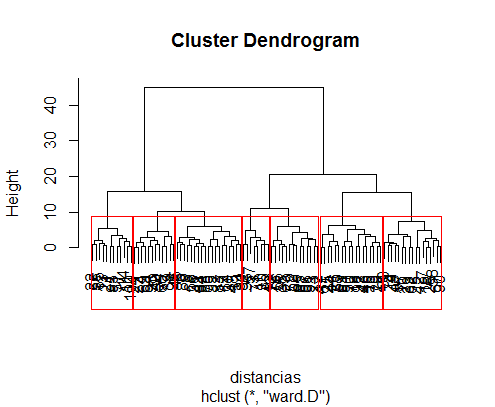
\includegraphics[scale=0.8]{cutree.png}
\end{center}
Utilizando las dos componentes principales para ver los clústers en dos dimensiones, el resultado es el siguiente:
\begin{center}
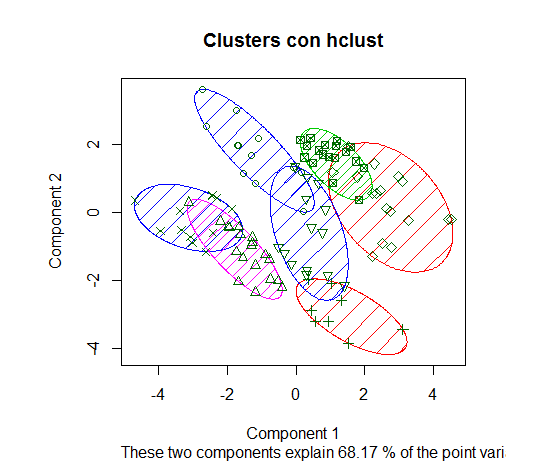
\includegraphics[scale=0.8]{clustershclust.png}
\end{center}
Cabe destacar que esta representación puede ser útil para ver la cantidad de elementos en cada clúster y que la separación entre ellos no es tanta. Sin embargo, dada la forma en que se realizó, esto no representa al $100\%$ la información de los clústers (en este caso sólo el $68.17\%$), por lo que se puede ver que hay una intersección en los grupos (cosa que en realidad no pasa) y no se pueden sacar mayores conclusiones sobre los elementos que componen cada uno.\\
\item[3.6)] Así, aplicando cutree y dividiendo en 7 grupos, obtenemos un vector donde en la coordenada i indica a qué clúster pertenece el individuo i, y se crea la nueva tabla.
\begin{verbatim}
> head(EjemploAlgoritmosRecomendacionHCLUST)
        X Velocidad.Entrega Precio Durabilidad Imagen.Producto Valor.Educativo
1    Adam              2.05   0.30        3.45            2.35             2.4
2    Anna              0.90   1.50        3.15            3.30             2.5
3 Bernard              1.70   2.60        2.85            3.00             4.3
4  Edward              1.35   0.50        3.55            2.95             1.8
5  Emilia              3.00   0.45        4.80            3.90             3.4
6  Fabian              0.95   1.65        3.95            2.40             2.6
  Servicio.Retorno Tamano.Paquete Calidad.Producto Numero.Estrellas Grupo
1              2.3           2.60             2.10              1.7     1
2              4.0           4.20             2.15              2.8     2
3              2.7           4.10             2.60              3.3     3
4              2.3           3.90             1.95              1.7     4
5              4.6           2.25             3.40              4.3     5
6              1.9           4.85             2.20              3.0     2
\end{verbatim}

\item[3.7)]Utilizando ahora el método de k-means, se hace la separación en 2 y 3 clústers. En el siguiente gráfico se muestran dichos clústers, representados por triángulos, círculos y cruces.
\begin{center}
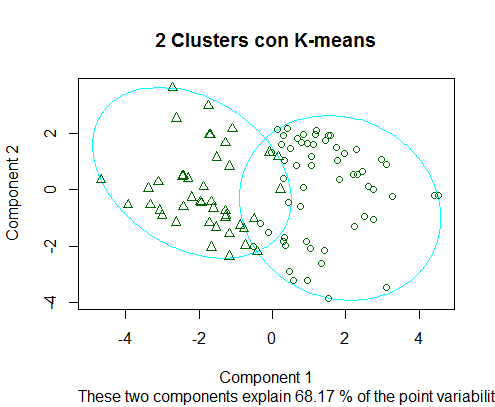
\includegraphics[scale=0.8]{kmeans2.png}
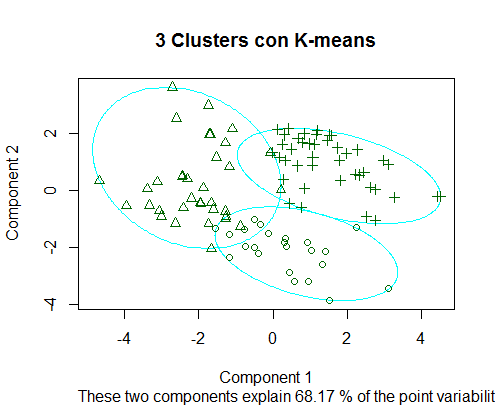
\includegraphics[scale=0.8]{kmeans3.png}
\end{center}
Cabe destacar que, como se mencionó anteriormente, se usó componentes principales para poder graficar estos clústers (en caso contrario no podrían verse en dos dimensiones), lo cual pueden no ser recomendable si no es alto el porcentaje de representación que tienen ambas componentes (en este caso, por ejemplo, se observan algunos triángulos mezclados con círculos o con cruces debido a lo mismo).\\
\\
Ahora, nuevamente se buscará cuál es el número óptimo de clústers con este método:

\begin{center}
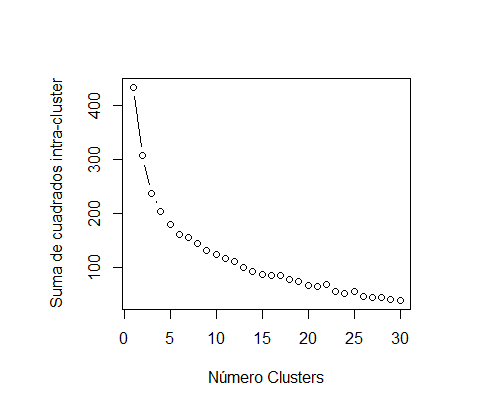
\includegraphics[scale=0.8]{codok.png}
\end{center}
Al igual que en el caso anterior, no hay un número de clústers que sea demasiado bueno, pero se optará por considerar 6, ya que con más clústers la diferencia cambiaría muy poco.\\
\begin{center}
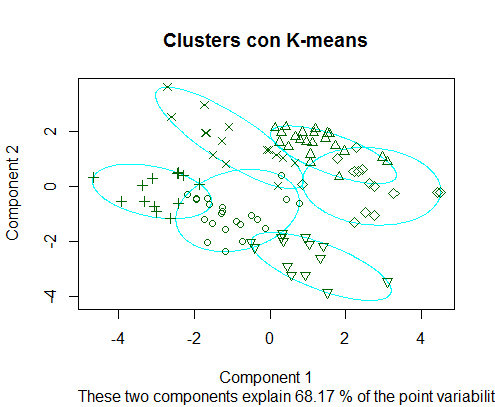
\includegraphics[scale=0.8]{kmeans6.png}
\end{center}
\item[3.8)]
Utilizando el número óptimo de clústers para clasificación jerárquica y k-means, graficamos los centros de gravedad de cada grupo formado, resultando lo siguiente:
\begin{center}
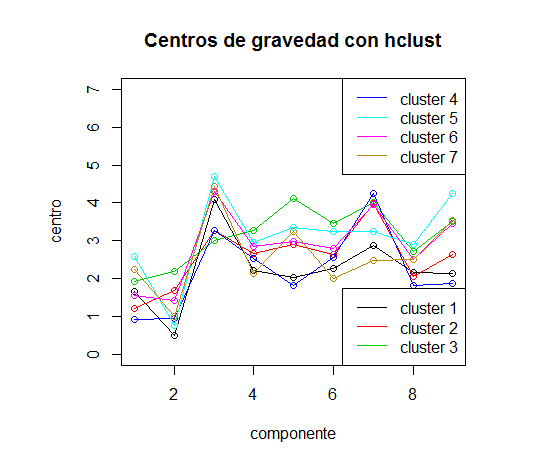
\includegraphics[scale=0.8]{centroshclust.png}
\end{center}
Notar que, tanto en este como en el gráfico siguiente, el eje x representa cada atributo de los individuos, es decir, cada columna de la tabla. De esta forma, 1 reprensenta la velocidad de entrega, 2 el precio, 3 la durabilidad, 4 la imagen del producto, 5 el valor educativo, 6 el servicio de retorno, 7 el tamaño del paquete, 8 la calidad del producto y 9 el número de estrellas.\\
\\
Aclarado esto, se observa que en el primer clúster están aquellos que evaluaron muy bien la durabilidad, regular (un poco mal o un poco bien) el tamaño del paquete, horrible el precio y mal lo demás. En el segundo están aquellos que evaluaron muy bien el tamaño del paquete, muy mal la velocidad de entrega, el precio y la calidad del producto y regular o levemente mal lo demás. En el tercero están quienes evaluaron muy bien el valor educativo y el tamaño del paquete, evaluaron bien o regular la imagen de producto, la durabilidad, el servicio de retorno y el número de estrellas y mal lo demás. En el cuarto están los que evaluaron excelente el tamaño del paquete, regular la durabilidad, horrible la velocidad de entrega y el precio y mal o muy mal lo demás. En el quinto están quienes evaluaron excelente la durabilidad y el número de estrellas, pésimo el precio y regular lo demás. En el sexto están quienes calificaron muy bien la durabilidad y el tamaño del paquete, muy mal la velocidad de entrega y el precio y bordean lo regular en lo demás (levemente mal o levemente bien). En el último están los que evalúan excelente la durabilidad, regular o bien el valor educativo y el número de estrellas, pésimo el precio y mal lo demás.

\begin{center}
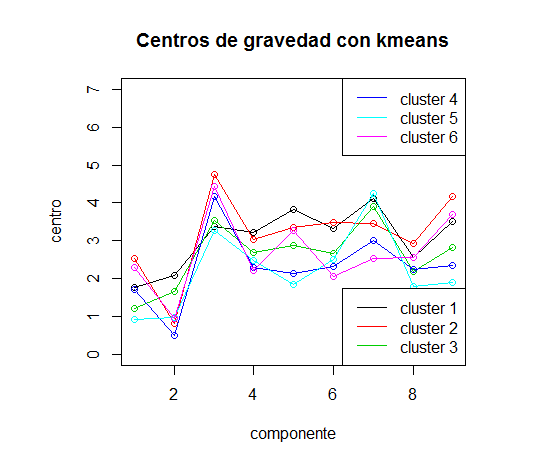
\includegraphics[scale=0.8]{centroskmeans.png}
\end{center}

En los conglomerados hechos por k-means se observa que en el primero están los individuos que calificaron regular o bien la durabilidad, la imagen del producto, el valor educativo, el servicio de retorno, el tamaño del paquete el número de estrellas y de mala forma las otras. Sin embargo, incluyendo a aquellos que tienen notas más centradas, es decir, donde las notas malas no sean tan malas y las buenas no demasiado buenas.\\
\\
En el segundo clúster están aquellos que calificaron de manera excelente la durabilidad y el número de estrellas, calificaron pésimo el precio, y todas las demás regular. En el tercero están quienes calificaron decente la durabilidad y el tamaño del paquete, calificaron mal (pero no muy mal) o regular la imagen de producto, el valor educativo, el servicio de retorno y el número de estrellas, calificaron mal la calidad del producto y muy mal la velocidad de entrega y el precio.\\
\\
En el cuarto grupo están quienes calificaron muy bien la durabilidad, calificaron pésimo el precio, decente el tamaño del paquete y mal lo demás (nuevamente, sin estar tan por debajo de lo regular). En el quinto están quienes calificaron excelente el tamaño del paquete, regular la durabilidad y mal lo demás, siendo horrible la velocidad de entrega y el precio. En el último están quienes evaluaron excelente la durabilidad, decente el valor educativo y el número de estrellas, pésimo el precio y mal lo demás.

\item[3.9)]Se busca en la tabla hecha con los clústers de clasificación jerárquica en el problema 3.6, y se ve que Teresa pertenece al primer grupo, Leo al sexto y Justin al séptimo. Así, a Teresa le recomendaría productos que tengan excelentes calificaciones en la durabilidad, a Leo productos que tengan muy buena puntuación de durabilidad y tamaño de paquete y a Justin productos que tengan muy buena nota en durabilidad y que estén al menos decente en el número de estrellas y el valor educativo.
\end{itemize}
\end{itemize}

\end{document}
